\documentclass[11pt,a4paper]{report}
\usepackage[spanish,es-nodecimaldot]{babel}	% Utilizar español
\usepackage[utf8]{inputenc}					% Caracteres UTF-8
\usepackage{graphicx}						% Imagenes
\usepackage[hidelinks]{hyperref}			% Poner enlaces sin marcarlos en rojo
\usepackage{fancyhdr}						% Modificar encabezados y pies de pagina
\usepackage{float}							% Insertar figuras
\usepackage[textwidth=390pt]{geometry}		% Anchura de la pagina
\usepackage[nottoc]{tocbibind}				% Referencias (no incluir num pagina indice en Indice)
\usepackage{enumitem}						% Permitir enumerate con distintos simbolos
\usepackage[T1]{fontenc}					% Usar textsc en sections
\usepackage{amsmath}						% Símbolos matemáticos

% Comando para poner el nombre de la asignatura
\newcommand{\asignatura}{Simulación de Sistemas}
\newcommand{\autor}{José María Sánchez Guerrero}
\newcommand{\titulo}{Práctica 1}
\newcommand{\subtitulo}{Diferentes Modelos de Simulación}

% Configuracion de encabezados y pies de pagina
\pagestyle{fancy}
\lhead{\autor{}}
\rhead{\asignatura{}}
\lfoot{Grado en Ingeniería Informática}
\cfoot{}
\rfoot{\thepage}
\renewcommand{\headrulewidth}{0.4pt}		% Linea cabeza de pagina
\renewcommand{\footrulewidth}{0.4pt}		% Linea pie de pagina

\begin{document}
\pagenumbering{gobble}

% Pagina de titulo
\begin{titlepage}

\begin{minipage}{\textwidth}

\centering


\includegraphics[scale=0.5]{img/ugr.png}\\

\textsc{\Large \asignatura{}\\[0.2cm]}
\textsc{GRADO EN INGENIERÍA INFORMÁTICA}\\[1cm]

\noindent\rule[-1ex]{\textwidth}{1pt}\\[1.5ex]
\textsc{{\Huge \titulo\\[0.5ex]}}
\textsc{{\Large \subtitulo\\}}
\noindent\rule[-1ex]{\textwidth}{2pt}\\[3.5ex]

\end{minipage}

\vspace{0.5cm}

\begin{minipage}{\textwidth}

\centering

\textbf{Autor}\\ {\autor{}}\\[2.5ex]
\textbf{Rama}\\ {Computación y Sistemas Inteligentes}\\[2.5ex]
\vspace{0.3cm}


\includegraphics[scale=0.3]{img/etsiit.jpeg}

\vspace{0.7cm}
\textsc{Escuela Técnica Superior de Ingenierías Informática y de Telecomunicación}\\
\vspace{1cm}
\textsc{Curso 2018-2019}
\end{minipage}
\end{titlepage}

\pagenumbering{arabic}
\tableofcontents
\thispagestyle{empty}				% No usar estilo en la pagina de indice

\newpage

\setlength{\parskip}{1em}

\chapter{Mi primer modelo de simulación de MonteCarlo}

Este modelo de simulación lo vamos a tratar con el problema del \textit{aparcamiento}, en el cual un coche se dispone
a aparcar a una distancia $x$ de su destino. También dispondremos de variables como el número de plazas que alcanza a
ver el conductor desde su posición o la probabilidad de que esa plaza esté ocupada o no. El ejercicio consiste en elegir
una plaza de aparcamiento $c$ en la cual el conductor, ni se quede muy corto ni se pase, es decir, que encuentre un
valor que minimice la distancia esperada desde el lugar de aparcamiento hasta el objetivo.


\section{Experimentación inicial}

Para hacernos una idea de los valores que obtendremos y los parámetros que más afectan al rendimiento de este modelo,
vamos a realizar una ejecución inicial del programa con todos los valores que trae por defecto.

Estos parámetros y sus valores son los siguientes:

\begin{itemize}
	\item Número de veces que se repite para hacer la media: 100000
	\item Posición de destino $x$: 100
	\item Número de posiciones siguientes que podemos ver: 2
	\item Probabilidad de que el aparcamiento esté ocupado: 0.9 (90\%)
\end{itemize}

El resultado de la ejecución es el siguiente: la mejor posicion inicial ha sido $c=94$ con una distancia media hasta
el destino de 6.50395 posiciones. Este resultado ya nos da una idea de cuáles van a ser los mejores valores $c$, y es que
cuanto más cerca empecemos a buscar aparcamiento, más se reducirá la distancia hasta el destino.

A continuación, vamos a mostrar una gráfica para poder comprobar esto que acabamos de decir y saber si estamos en lo
cierto o no.

\begin{figure}[H]
\centering
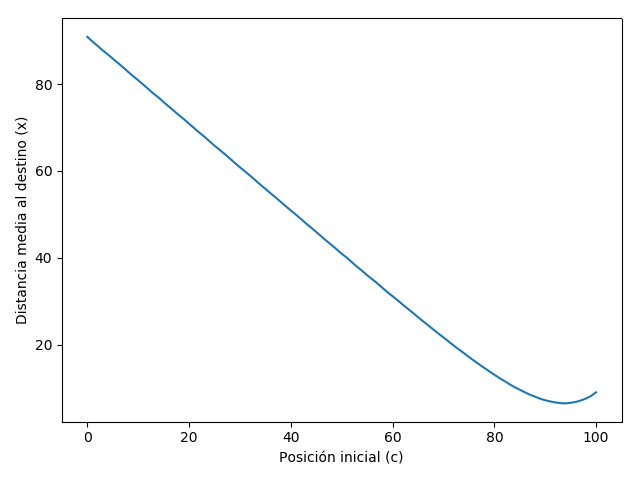
\includegraphics[scale=0.7]{img/x-100-2-90.png}
\caption{Valor medio de la distancia a medida que nos acercamos a $x=100$}
\end{figure}

Como podemos ver en la gráfica, se cumple lo que habíamos mencionado. Esto se debe a que nos quedamos con el primer
sitio que encontramos, y si empezamos a buscar desde una plaza muy alejada del destino, terminaremos aparcando en
una plaza bastante alejada también.

En la gráfica también vemos que a partir de $c=94$ se aumenta la distancia al destino, ya que probablemente no encuentre
ninguna posición cercana al destino y se pase. Esto nos hace pensar que, pese a que el $c=94$ sea la mejor plaza teniendo
en cuenta únicamente la media, puede dar unos resultados muy diferentes, es decir, que puede tener una varianza más alta
respecto a otras posiciones.

Al igual que hemos hecho con la distancia al destino, a continuación vamos a mostrar una gráfica conlos valores que nos
ofrece la desviación típica y los mejores resultados.

\begin{figure}[H]
\centering
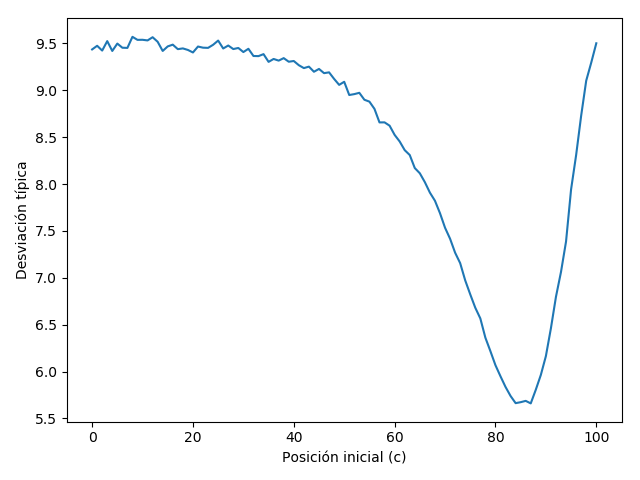
\includegraphics[scale=0.7]{img/dt-100-2-90.png}
\caption{Valor medio de las desviaciones típicas a medida que nos acercamos a $x=100$}
\end{figure}

El resultado de la ejecución es el siguiente: la posicion inicial con menos desviación típica ha sido $c=84$ con un valor
medio de 5.651982. Por lo que podemos ver en la gráfica, para los valores que hay alrededor del $c=94$, que es el que
menor distancia al destino tenía, tiene unos valores de desviación típica más altos. Esto nos confirma que, efectivamente,
empezar a buscar tan cerca del destino nos puede salir en ocasiones muy bien pero en otras no tanto.


\section{Experimentación modificando los parámetros}

En este apartado vamos a ver que sucede cuando modificamos los parámetros de nuestro modelo y cómo afectan al comportamiento
del sistema. 

\subsection{Posición de destino}

Vamos a comenzar modificando la posición de destino, dándole por ejemplo un valor de \textbf{x=50} y otro de \textbf{x=200}.
El resultado de la ejecución es el siguiente.

\newpage

Para \textbf{x=50} el resultado de la ejecución nos dice que la mejor posicion inicial ha sido $c=44$ con una distancia media hasta
el destino de 6.50545 posiciones; y en cuanto a la desviación típica, que la posicion inicial que ha obtenido un valor más
bajo sido $c=35$ con una media de 5.646533.

A continuación, las dos gráfica correspondientes a los resultados:

\begin{figure}[H]
\centering
\begin{minipage}{0.5\textwidth}
  \centering
  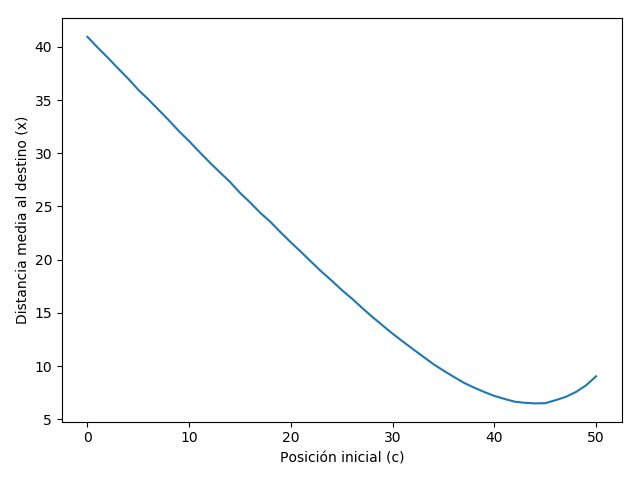
\includegraphics[scale=0.4]{img/x-50-2-90.png}
\end{minipage}%
\begin{minipage}{0.5\textwidth}
  \centering
  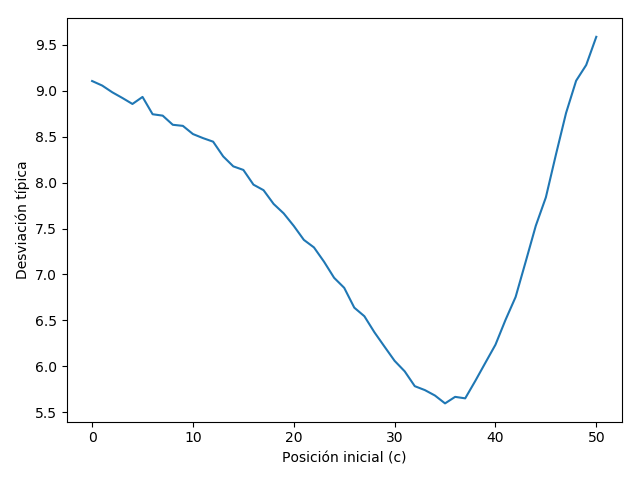
\includegraphics[scale=0.4]{img/dt-50-2-90.png}
\end{minipage}
\caption{Valores medios de las distancias y las desviaciones típicas a medida que nos acercamos a x = 50}
\end{figure}

Podemos ver que la posición $c$ en la que se empieza a buscar aparcamiento lógicamente ha cambiado, ya que no tenemos tantas
plazas como teníamos anteriormente. Sin embargo, observando los valores medios de la distancia y de la desviación típica,
podemos observar como son muy parecidos a los que ya teníamos (incluso el valor de $c$ con la menor desviación típica está
aproximadamente 10 por debajo del que tienen las distancias).

Si nos fijamos en las gráficas, vemos que son muy similares a las que obtuvimos en la primera ejecución, y por tanto, podemos
confirmar que este parámetro no influye demasiado en el modelo.

Vamos a ver ahora que sucede con un \textbf{x=200}. El resultado de la ejecución nos dice que la mejor posicion inicial ha sido
$c=194$ con una distancia media hasta el destino de 6.46297 posiciones; y en cuanto a la desviación típica, que la posicion
inicial que ha obtenido un valor más bajo sido $c=187$ con una media de 5.60064.

\begin{figure}[H]
\centering
\begin{minipage}{0.5\textwidth}
  \centering
  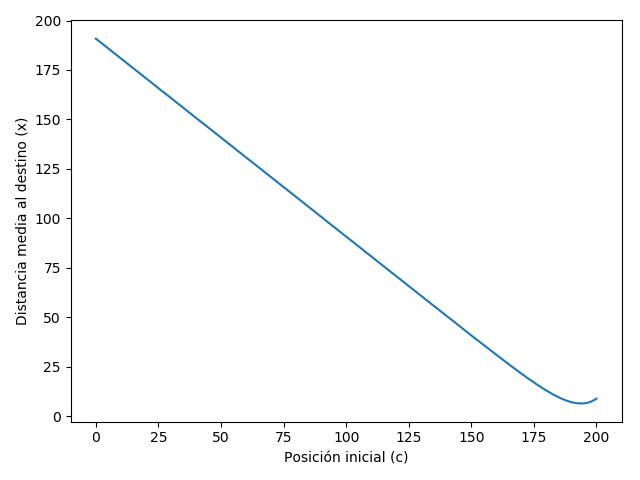
\includegraphics[scale=0.4]{img/x-200-2-90.png}
\end{minipage}%
\begin{minipage}{0.5\textwidth}
  \centering
  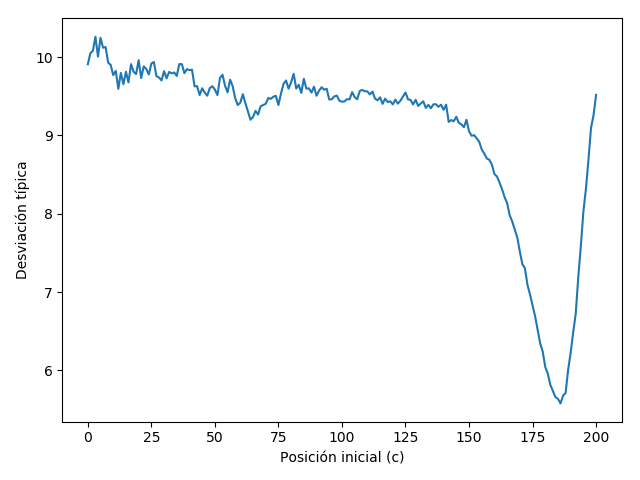
\includegraphics[scale=0.4]{img/dt-200-2-90.png}
\end{minipage}
\caption{Valores medios de las distancias y las desviaciones típicas a medida que nos acercamos a x = 200}
\end{figure}

Al igual que en las otras ejecuciones, tanto los resultados como las gráficas también son muy similiares (los valores cambian
la forma de la curva, pero el patrón que siguen es muy parecido), lo cual nos sirve para asegurar todavía más lo comentado
anteriormente.

\subsection{Número de posiciones vistas}

El siguiente parámetro que vamos a modificar va a ser el número de posiciones que vamos a poder ver desde la que nos encontramos.
Este parámetro tiene por defecto un valor de 2, por lo que vamos a probar por ejemplo con 0 y con 10. El resto de parámetros los
dejaremos como estaban en un principio.

El resultado de las simulaciones con estos parámetros son los siguientes:
\begin{itemize}[label=\textbullet]
	\item Para \textbf{vision=0} la mejor posicion inicial ha sido $c=94$ con una distancia media hasta el destino de 6.54038posiciones;
	y la mejor desviación típica, se ha obtenido en $c=86$ con una media de 5.642444.
	\item Para \textbf{vision=10} la mejor posicion inicial ha sido $c=92$ con una distancia media hasta el destino de 5.65583 posiciones;
	y la mejor desviación típica, se ha obtenido en $c=85$ con una media de 5.448542.
\end{itemize}

En este caso vemos cómo la distancia media hasta el destino se está reduciendo a medida que aumentamos el número de posiciones que
observamos desde el vehículo. No obstante, las desviaciones típicas, pese a que se han reducido un poco, el cambio tampoco es muy grande.

Vamos a mostrar las gráficas de estas dos ejecuciones a ver si podemos ver algo más relevante en ellas.

\begin{figure}[H]
\centering
	\begin{minipage}{0.5\textwidth}
	  \centering
	  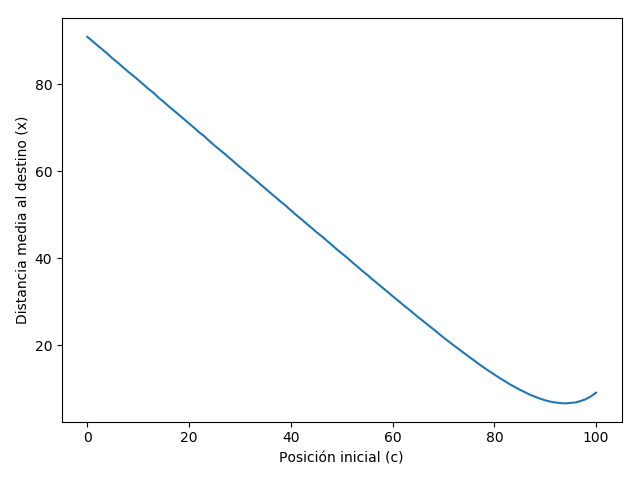
\includegraphics[scale=0.4]{img/x-100-0-90.png}
	\end{minipage}%
	\begin{minipage}{0.5\textwidth}
	  \centering
	  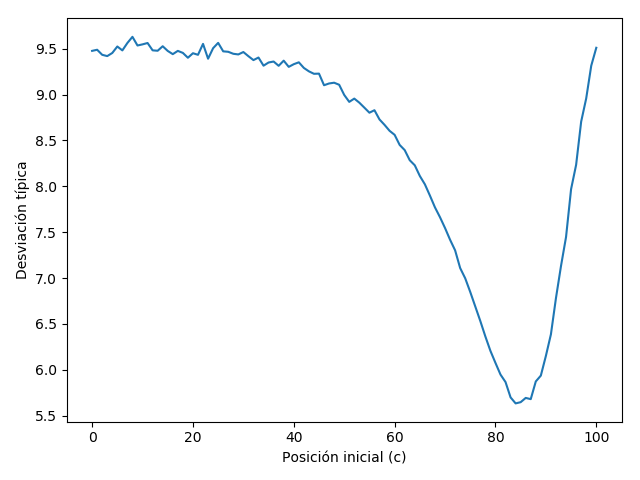
\includegraphics[scale=0.4]{img/dt-100-0-90.png}
	\end{minipage}
\caption{Valores medios de las distancias y las desviaciones típicas con visión=0}
\end{figure}

\begin{figure}[H]
	\begin{minipage}{0.5\textwidth}
	  \centering
	  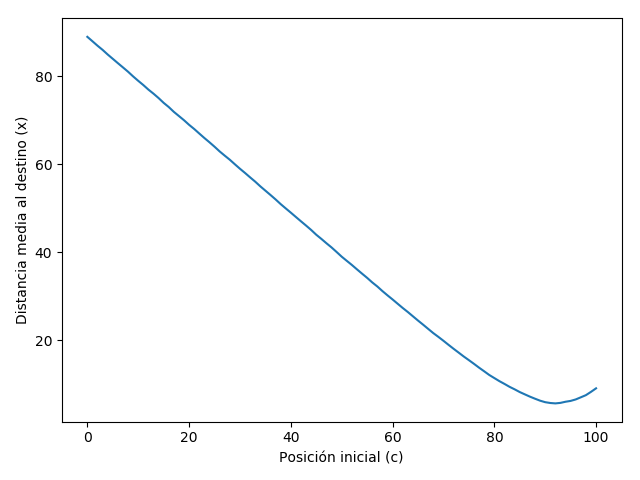
\includegraphics[scale=0.4]{img/x-100-10-90.png}
	\end{minipage}
	\begin{minipage}{0.5\textwidth}
	  \centering
	  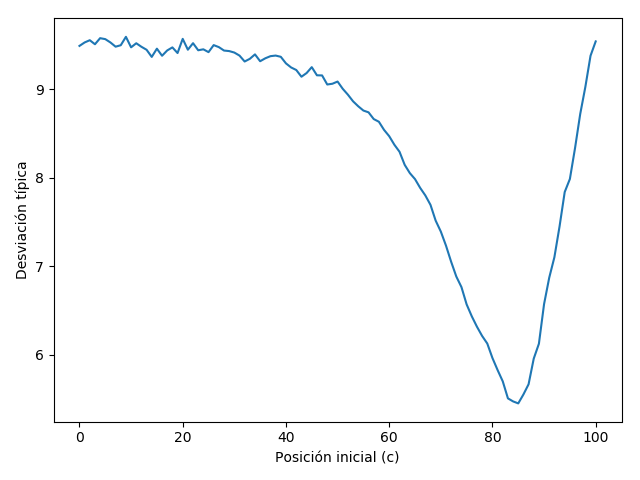
\includegraphics[scale=0.4]{img/dt-100-10-90.png}
	\end{minipage}
	\caption{Valores medios de las distancias y las desviaciones típicas con vision=10}
\end{figure}

Podemos ver que las gráficas siguen la misma tendencia que las gráficas de la ejecución por defecto y las del apartado anterior,
lo cual nos dice que, aun cambiando este parámetro, cuanto más cerca empecemos a buscar aparcamiento, más se reducirá la distancia
hasta el destino.

Sin embargo, con las gráficas no se puede apreciar bien cuánto se llega a reducir esta distancia, algo que si
apreciamos con valores numéricos, asi que voy a realizar otra ejecución con un abanico de valores más amplio para este parámetro.

\newpage

A continuación, una tabla con el resultado de esta ejecución:

\begin{table}[H]
\centering
\begin{tabular}{c|cc}
\textbf{Visión} & \textbf{Mejor posición inicial} & \textbf{Mejor distancia} \\ \hline
\textbf{0}      & 94                              & 6.55275                  \\ \hline
\textbf{5}      & 94                              & 6.29162                  \\ \hline
\textbf{10}     & 92                              & 5.64137                  \\ \hline
\textbf{15}     & 89                              & 5.26576                  \\ \hline
\textbf{20}     & 86                              & 5.03522                  \\ \hline
\textbf{25}     & 83                              & 4.9281                   \\ \hline
\textbf{30}     & 82                              & 4.82683                  \\
\end{tabular}
\end{table}

Como podemos observar, la mejor posición inicial es cada vez más lejana al destino, no obstante, la mejor distancia media también
se está reduciendo. Esto se debe a que, contra más visión se tenga de los aparcamientos que tenemos delante, no necesitaremos avanzar
hasta posiciones cercanas a nuestro destino, porque ya sabremos si hay aparcamiento o no.

\subsection{Probabilidad de encontrar aparcamiento}

Este parámetro sería el único que tiene aleatoriedad, ya que en un problema de la vida real, podemos saber dónde está nuestro destino
o el número de aparcamientos que somos capaces de ver, pero nunca tendremos control sobre la cantidad de aparcamiento libres que hay
en una calle.

Por esta razón, este parámetro será el que más merezca la pena estudiar. Vamos a comenzar sacando una tabla similar a la del apartado
anterior, ya que se pueden ver con más detalle los valores obtenidos en la ejecución.

\begin{table}[H]
\centering
\begin{tabular}{c|cc}
\textbf{\% de ocupación} & \textbf{Mejor posición inicial} & \textbf{Mejor distancia} \\ \hline
\textbf{25}     		 & 99                              & 0.273390                 \\ \hline
\textbf{50}     		 & 99                              & 0.743700                 \\ \hline
\textbf{75}     		 & 98                              & 2.162840                 \\ \hline
\textbf{80}     		 & 97                              & 2.955510                 \\ \hline
\textbf{85}     		 & 96                              & 4.138430                 \\ \hline
\textbf{90}     		 & 94                              & 6.494790                 \\ \hline
\textbf{95}     		 & 87                              & 13.458690                \\
\end{tabular}
\end{table}

Como podemos observar en la tabla, cuanto más bajo es el porcentaje de ocupación, más fácil es encontrar aparcamiento, y por tanto,
la distancia media a la que aparcamos es también muy baja. A medida que vamos aumentando este porcentaje, vemos como la posicion
inicial a la que se empieza a buscar aparcamiento está más lejos y, en cosecuencia, la mejor distancia aumenta.

Por último, vamos a mostrar una gráfica que muestra tres porcentajes de ocupación distintos para observar cómo cambia la distancia
entre ellos.

\begin{figure}[H]
\centering
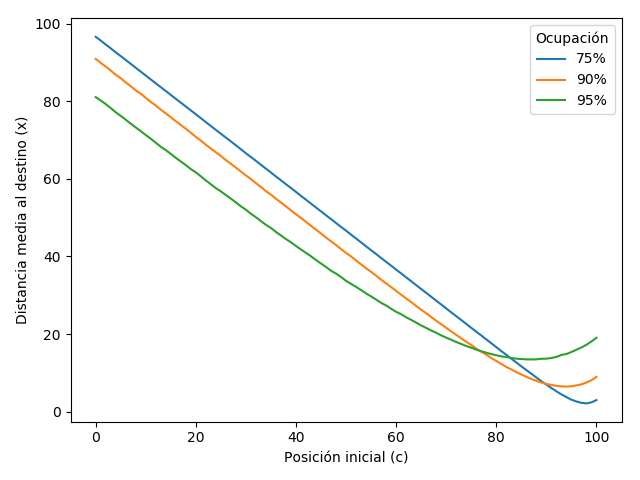
\includegraphics[scale=0.6]{img/x-100-2-75.png}
\caption{Valores medios de la distancias con distintos porcentajes de ocupación}
\end{figure}

\begin{figure}[H]
\centering
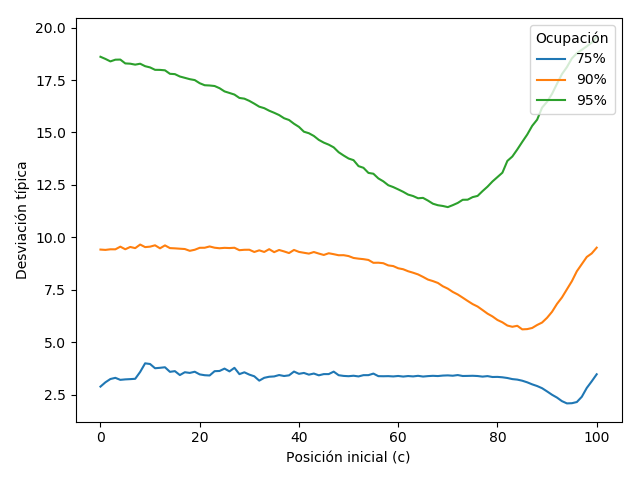
\includegraphics[scale=0.6]{img/dt-100-2-75.png}
\caption{Valores de la desviación típica con distintos porcentajes de ocupación}
\end{figure}

En la primera gráfica vemos cómo para un porcentaje bajo de ocupación, los valores de la gráfica llegan a sus mínimos cuando
se aproximan a $c=100$, porque da igual lo tarde que empiece a buscar un aparcamiento si las probabilidades de que encuentre
uno libre son bastante altas. Por otra parte, con un porcentaje de ocupación más alto, la distancia que tiene que recorrer
no es tan baja como antes, ya que si la posición inicial es cercana al destino la probabilidad de que se pase es más alta.

Esto último lo podemos corroborar con la gráfica de las desviaciones típicas, en la cual vemos cómo para estos altos porcentajes
de ocupación, la línea es mucho más pronunciada y ocupa unos valores más altos en comparación a los bajos porcentajes de ocupación.
Es decir, que cuanta más ocupación exista, es más propenso a pasarse del destino y a que las distancias aumenten.


\section{Experimentación con varios parámetros y valores extremos}

En esta sección no vamos a analizar todas y cada una de las posibilidades que tenemos, ni lo vamos a hacer tan en profundidad
como lo hicimos anteriormente, ya que nos podríamos extender demasiado.

Lo primero a tener en cuenta es, que la posición de destino $x$ la vamos a mantener en todas las ejecuciones como 100, porque
como hemos visto, es un parámetro muy poco relevante para la simulación. Dicho esto, pasemos a comentar cómo vamos a proceder
en esta experimentación.

Los parámetros a tener en cuenta serán:
\begin{itemize}[label=\textbullet]
	\item \textbf{Visión.} Que lo variaremos entre 0 y 100 para probar todas las posibilidades hasta llegar a valores extremos
	como el 100 que nos permitan ver todos los aparcamientos
	\item \textbf{Porcentaje de ocupación.} Que irá desde el 50\% hasta un $\approx100\%$, ya que el máximo hace que obtengamos
	un error (lógicamente, si todos los aparcamiento están ocupados, el programa buscará uno libre hasta que se quede sin memoria).
\end{itemize}

\newpage

En la siguiente tabla podemos observar los resultados de combinar todos los parámetros:

\begin{table}[H]
\centering
\begin{tabular}{c|c|c|c}
\textbf{Visión} & \textbf{\% de ocupación} & \textbf{Mejor posición inicial} & \textbf{Mejor distancia} \\ \hline
\textbf{2}      & \textbf{50}              & 98                              & 0.747980                 \\ \hline
\textbf{10}     & \textbf{50}              & 94                              & 0.662560                 \\ \hline
\textbf{50}     & \textbf{50}              & 90                              & 0.662040                 \\ \hline
\textbf{100}    & \textbf{50}              & 40                              & 0.659470                 \\ \hline
\textbf{2}      & \textbf{75}              & 98                              & 2.155360                 \\ \hline
\textbf{10}     & \textbf{75}              & 94                              & 1.766020                 \\ \hline
\textbf{50}     & \textbf{75}              & 73                              & 1.701890                 \\ \hline
\textbf{100}    & \textbf{75}              & 56                              & 1.698420                 \\ \hline
\textbf{2}      & \textbf{90}              & 94                              & 6.527760                 \\ \hline
\textbf{10}     & \textbf{90}              & 91                              & 5.662930                 \\ \hline
\textbf{50}     & \textbf{90}              & 72                              & 4.743880                 \\ \hline
\textbf{100}    & \textbf{90}              & 36                              & 4.712600                 \\ \hline
\textbf{2}      & \textbf{99}              & 31                              & 68.768227                \\ \hline
\textbf{10}     & \textbf{99}              & 34                              & 68.632362                \\ \hline
\textbf{50}     & \textbf{99}              & 30                              & 67.091072                \\ \hline
\textbf{100}    & \textbf{99}              & 18                              & 60.555672                \\ \hline
\end{tabular}
\end{table}

Analizando los valores que hemos obtenido, podemos ver como, pese a que el número de posiciones que vemos '\textit{Visión}' reduce
ligeramente la distancia, a lo que realmente afecta es a la posición inicial a partir de la cual empezamos a buscar aparcamiento.
Esto se debe lógicamente a la capacidad que tenemos de ver los siguientes aparcamientos, y en el caso de valores extremos (como es
el caso de verlos todos $vision=100$) obtenemos los valores más bajos.

En cuanto al porcentaje de ocupación, sin duda es el parámetro que más influye en la distancia a la que aparcaremos de nuestro
destino, ya que la mejora que se puede llegar a conseguir entre un 50\% de ocupación y un 99\% de ella es de aproximadamente 68
posiciones; mientras que la máxima mejora que se consigue gracias a la visión, es de aproximadamente de 8 posiciones. Incluso si
nos fijamos en la última fila de la tabla (donde tenemos los dos parámetros con valores extremos), podemos ver cómo ni teniendo
toda la visión de la calle, conseguimos bajar a un valor considerable la distancia.



\chapter{Mi primer modelo de simulación discreto}

Para este modelo de simulación utilizaremos un problema llamado \textit{radares}, en el que tendremos varios radares funcionando y
al cabo del tiempo una de sus componentes se romperá, teniendo que reemplazarla por repuestos que tendremos almacenados. En caso
de que nos quedemos sin repuestos, el radar se quedará fuera de servicio.

Los parámetros que se le pueden pasar a este programa son los siguientes (con sus valores por defecto):
\begin{itemize}
	\item Número de radares que hay "\textit{radares}": 5
	\item Número de repuestos almacenados "\textit{disponibles}": por determinar
	\item Tiempos mínimo y máximo de devolción de componentes reparados "\textit{vmin}" y "\textit{vmax}": 15 y 30
	\item Tiempo entre fallos "\textit{tfallo}": 20
	\item Tiempo total a simular "\textit{tiempo\_total}": 365 (un año)
	\item Número de simulaciones "\textit{simulaciones}":por determinar
\end{itemize}

Tendremos que realizar dos experimentos. El primero que investigue el número mínimo de componentes que habría que tener para no
tener el espacio aéreo desprotegido; y el segundo será un análisis de cómo influyen los distintos parámetros en el rendimiento del
sistema.


\section{Experimentación para el número de repuestos}

En este ejemplo, únicamente tendremos que determinar nosotros el número de simulaciones y el número de repuestos almacenados. El
resto los dejaremos tal y como están, por defecto.

En primer lugar, vamos a determinar el número mínimo de radares que tendremos que tener, el cual lo determinaremos con un $simulaciones
=1000$, ya que es un valor suficientemente grande para obtener unos buenos resultados de media. Aun asi, posteriormente, veremos que
pasa cambiando este parámetro.

Vamos a realizar una ejecución para un número de radares de repuesto que va de 5 a 20. Estos son los resultados que hemos obtenido:

\begin{table}[H]
\centering
\resizebox{\textwidth}{!}{%
\begin{tabular}{c|c|c}
\textbf{Radares} & \textbf{\begin{tabular}[c]{@{}c@{}}Media del porcentaje\\ del tiempo desprotegido\end{tabular}} & \textbf{\begin{tabular}[c]{@{}c@{}}Desviación típica del\\ porcentaje del tiempo desprotegido\end{tabular}} \\ \hline
\textbf{5}	     & 37.0384                             & 8.39283                 \\ \hline
\textbf{6}  	 & 24.8135                             & 7.50727                 \\ \hline
\textbf{7}     	 & 15.1238                             & 6.04561                 \\ \hline
\textbf{8}     	 & 8.85408                             & 5.00746                 \\ \hline
\textbf{9}     	 & 4.76202                             & 3.41032                 \\ \hline
\textbf{10}      & 2.28223                             & 2.30909                 \\ \hline
\textbf{11}      & 0.933034                            & 1.42739                 \\ \hline
\textbf{12}      & 0.460005                            & 0.950908                \\ \hline
\textbf{13}      & 0.162082                            & 0.535298                \\
\end{tabular}%
}
\end{table}

Vemos que a partir de 11 radares almacenados, la media del porcentaje ya es inferior al 1\%, sin embargo, como podemos ver en el valor de
la desviación típica, es relativamente alto. Esto quiere decir que, pese a que la media nos ha salido por debajo del umbral, han habido
bastantes ejecuciones en las que sí lo ha superado. Si probamos con 12 radares, tenemos una situación parecida, ya que la media nos sale
por debajo del umbral, pero la desviación tipica también es bastante alta. Quizás no lo hace por mucho, pero para más seguridad yo
almacenaría un radar más, ya que tampoco será un coste muy alto y tengo la certeza de que no superará el umbral o  lo hará en muy pocas
ocasiones.

Una vez ya hemos encontrado unos valores para el número de radares almacenados, vamos a comentar que sucede si cambiamos el número
de simulaciones. Si probamos con un número de simulaciones alto, como puede ser 1000 (el que ya emos utilizado), 500 o 100; podremos
decir que el experimento es bastante bueno, ya que la media será bastante representativa.

\newpage

Sin embargo, veamos lo que puede pasar con un número bajo de ejecuciones:
\begin{figure}[H]
\centering
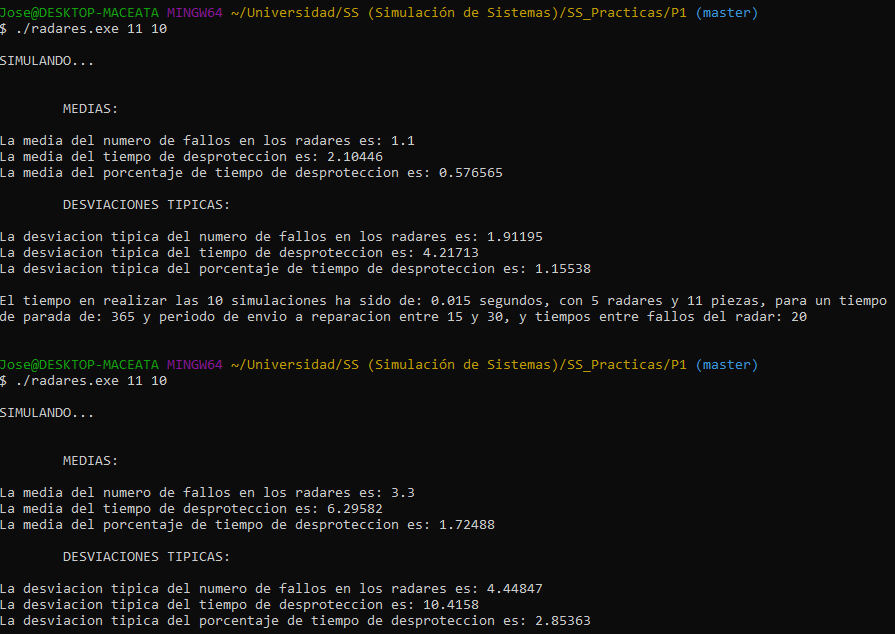
\includegraphics[scale=0.38]{img/sim10_radares.png}
\caption{Ejecución con 10 simulaciones.}
\end{figure}

Como podemos observar, con 11 radares no nos ha costado mucho obtener, tanto una simulación que pasa del 1\%, como otra que obtiene valores
por debajo. Esto quiere decir que, como tenemos ciertas variables aleatorias no obtenemos un resultado válido con un número tan bajo de
ejecuciones, es decir, no ofrece una media representativa del modelo.

Si probamos ahora con un número de simulaciones aun más bajo, vemos que el resultado varía todavía más:
\begin{figure}[H]
\centering
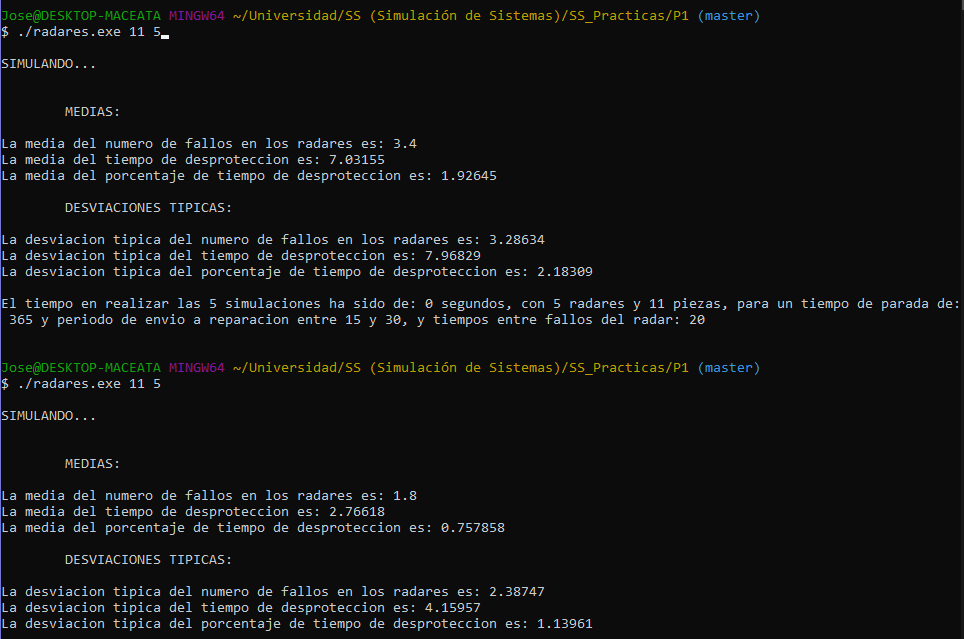
\includegraphics[scale=0.38]{img/sim5_radares.png}
\caption{Ejecución con 5 simulaciones.}
\end{figure}


\section{Influencia en el rendimiento de los parámetros}

En esta sección analizaremos cómo cambia el rendimiento del sistema modificando sus parámetros internos, como pueden ser tanto acortar
el tiempo de devolución de componentes reparados o emplear componentes con más tiempo de vida.

Vamos a empezar cambiando el tiempo de devolución. Por defecto en la simulación tardan entre 15 y 30 días, asi que nosotros podemos probar
reduciendo este tiempo en, por ejemplo, 10 días. Comentar antes de mostrar los resultados, que para el resto de parámetros pondremos los
que vienen por defecto (excepto el número de repuestos, que estamos optimizando) y el número de simulaciones a 1000, ya que es el más
representativo y no tarda demasiado en ejecutarse.

\begin{table}[H]
\centering
\resizebox{\textwidth}{!}{%
\begin{tabular}{c|c|c}
\textbf{Radares} & \textbf{\begin{tabular}[c]{@{}c@{}}Media del porcentaje\\ del tiempo desprotegido\end{tabular}} & \textbf{\begin{tabular}[c]{@{}c@{}}Desviación típica del\\ porcentaje del tiempo desprotegido\end{tabular}} \\ \hline
\textbf{5}	     & 8.03518                             & 3.88919                 \\ \hline
\textbf{6}  	 & 3.42126                             & 2.46856                 \\ \hline
\textbf{7}     	 & 1.24311                             & 1.37181                 \\ \hline
\textbf{8}     	 & 0.440921                            & 0.776739                \\ \hline
\textbf{9}     	 & 0.128418                            & 0.402314                \\
\end{tabular}%
}
\end{table}

Podemos ver en estos resultados que, los resultados que anteriormente obteníamos con 12-13 radares aproximadamente, ahora los conseguimos
con 8-9 radares. Esto quiere decir que la simulación está bien hecha, ya que lo lógico al reducir el tiempo de devolución, tengamos un
porcentaje de tiempo desprotegido inferior. También nos hace cuestionarnos si merece la pena o no, pagar el precio que valdría una devolución
más rápida o invertir más en piezas (incluso podríamos plantearnos en reducir aun más el tiempo de devolución, si fuese posible).

A continuación, modificaremos el tiempo de vida de los componentes, es decir, vamos a comprobar si merece la pena gastar más dinero en
emplear componentes más robustos. El tiempo de vida que tenemos por defecto es de aproximadamente 20 días, asi que vamos a aumentarlo en
10 días y comprobamos que sucede.

\begin{table}[H]
\centering
\resizebox{\textwidth}{!}{%
\begin{tabular}{c|c|c}
\textbf{Radares} & \textbf{\begin{tabular}[c]{@{}c@{}}Media del porcentaje\\ del tiempo desprotegido\end{tabular}} & \textbf{\begin{tabular}[c]{@{}c@{}}Desviación típica del\\ porcentaje del tiempo desprotegido\end{tabular}} \\ \hline
\textbf{5}	     & 14.1074                            & 6.39146              \\ \hline
\textbf{6}  	 & 7.12183                            & 4.6315               \\ \hline
\textbf{7}     	 & 3.11415                            & 2.80384              \\ \hline
\textbf{8}     	 & 1.20292                            & 1.80842              \\ \hline
\textbf{9}     	 & 0.486128                           & 1.05936              \\
\end{tabular}%
}
\end{table}

Vemos que aumentar el tiempo de vida a un mes (10 días más) también nos mejora los resultados por defecto. Volvemnos a plantearnos el mismo
dilema de antes, y es si nos merece la pena aumentar el presupuesto en piezas más duradera o invertir en más cantidad. Aqui podemos ver que
siendo un poco mejores, ya podríamos utilizar 9 repuestos aproximadamente.

No obstante, veamos que sucede si cambiamos los dos parámetros que acabamos de cambiar en una misma simulación.

\begin{table}[H]
\centering
\resizebox{\textwidth}{!}{%
\begin{tabular}{c|c|c}
\textbf{Radares} & \textbf{\begin{tabular}[c]{@{}c@{}}Media del porcentaje\\ del tiempo desprotegido\end{tabular}} & \textbf{\begin{tabular}[c]{@{}c@{}}Desviación típica del\\ porcentaje del tiempo desprotegido\end{tabular}} \\ \hline
\textbf{5}	     & 1.81117                             & 1.7544                 \\ \hline
\textbf{6}  	 & 0.493805                            & 0.872734               \\ \hline
\textbf{7}     	 & 0.103228                            & 0.344626               \\ \hline
\textbf{8}     	 & 0.0213589                           & 0.142657               \\ \hline
\textbf{9}     	 & 0.00386476                          & 0.0482657              \\
\end{tabular}%
}
\end{table}

Los valores ya son muy bajos aún con 5 radares, pero para entrar en el umbral permitido tendríamos que tener almacenados entre 6-7 repuestos,
los cuales son prácticamente la mitad de repuestos que teníamos en la simulación inicial.

Partiendo de que estos componentes son muy caros, yo preferiría invertir un poco más en reducir costes de devolución y en aumentar la calidad
del producto, ya que estamos hablando de tener la mitad de estos (sale a casi un repuesto por radar). Esto es simple especulación, ya que no
disponemos de los precios exactos de cada parámetro, pero en caso de tenerlos se podría hacer un estudio aun más completo.



\chapter{Mi primer modelo de simulación continuo}

Este modelo de simulación lo estudiaremos con el problema \textit{Simulacion\_lago 2especiespeces}, en el que tendremos que introducir una
cantidad de peces inicial en un lago, grandes y pequeños, y veremos cómo evoluciona la población en diferentes instantes de tiempo. Hay
que tener en cuenta varias cosas, como la tasa de crecimiento, que los peces grandes comen unos 10 peces pequeños cada día o que el
lago tiene una capacidad máxima de 10000000 de peces pequeños y 36000 grandes. Posteriormente, también estudiaremos cómo afectaría una
campaña de pesca y regularemos un política.


\section{Estabilizar el sistema}

Para comenzar, vamos a intentar que el sistema alcance un punto estable de equilibrio para cada especie. Tendremos que simular varios años
para que se vea correctamente la evolución, asi que yo optaré por poner 20 (o 7300 días); y en cuanto a la cantidad de peces, una que impida
que los peces grandes extingan a los pequeños, pero sin tener que meter una cantidad exagerada de estos, ya que su tasa de crecimiento es
tres veces mayor.

Vamos a poner en un principio 25 peces grandes y ajustaremos el valor de los pequeños en base a estos. Empecemos poniendo un valor de 1000
peces pequeños y mostremos en una gráfica el resultado.

\begin{figure}[H]
	\begin{minipage}{0.5\textwidth}
	  \centering
	  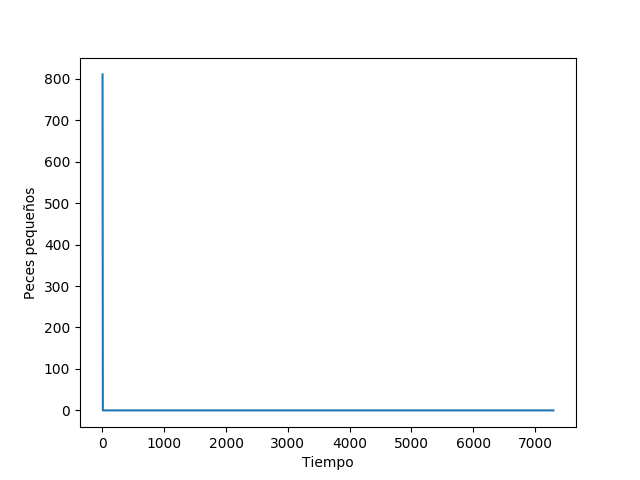
\includegraphics[scale=0.45]{img/pequenios-800-25.png}
	\end{minipage}
	\begin{minipage}{0.5\textwidth}
	  \centering
	  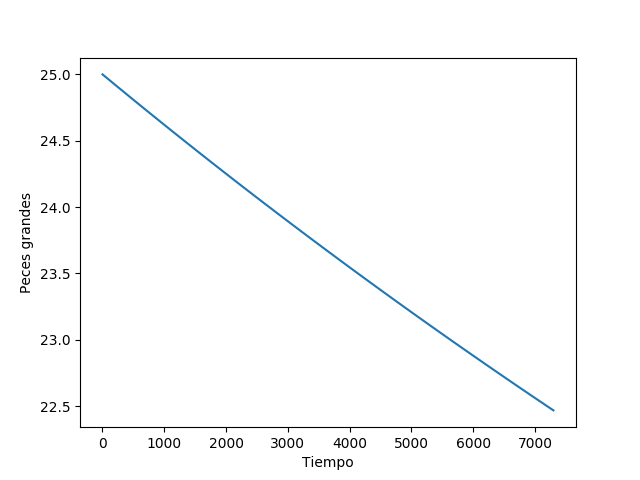
\includegraphics[scale=0.45]{img/grandes-800-25.png}
	\end{minipage}
	\caption{Evolución de la población de peces en 7300 días con pequeños: 1000 y grandes: 25.}
\end{figure}

Como podemos comprobar, esta cantidad de peces pequeños es muy baja, por lo que rápidamente han desaparecido, mientras que los grandes, al
cabo del tiempo, también lo han ido haciendo por falta de comida. Esto quiere decir que necesitamos meter más peces pequeños desde el principio,
asi que probemos con unos 4000. Este el el resultado:

\begin{figure}[H]
	\begin{minipage}{0.5\textwidth}
	  \centering
	  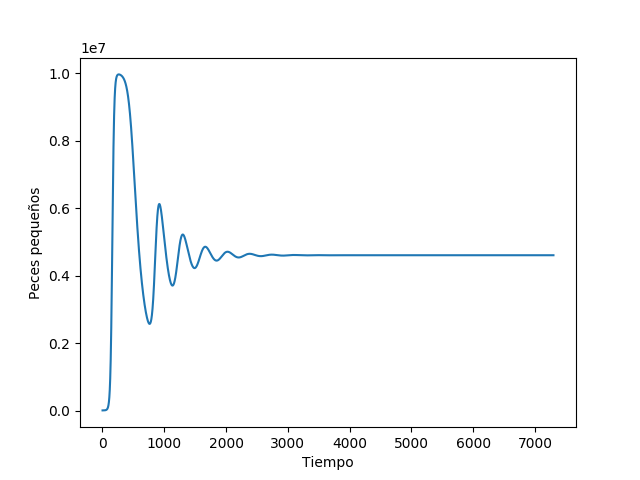
\includegraphics[scale=0.45]{img/pequenios-4000-25.png}
	\end{minipage}
	\begin{minipage}{0.5\textwidth}
	  \centering
	  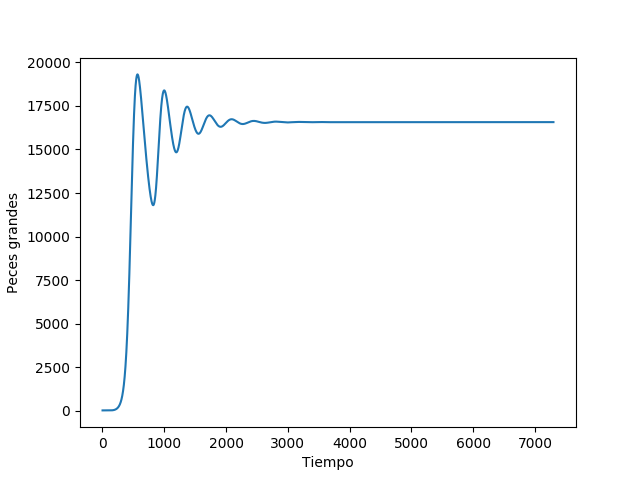
\includegraphics[scale=0.45]{img/grandes-4000-25.png}
	\end{minipage}
	\caption{Evolución de la población de peces en 7300 días con pequeños: 4000 y grandes: 25}
\end{figure}

En este caso sí podemos cómo, alrededor de los 2000 días, los dos tipos de peces han conseguido estabilizarse, llegando a punto en el que su
población no varía. También podemos observar cómo ha aumentado considerablemente el número de peces, llegando los pequeños a los 70 millones
y los grandes a los 20.000; y por eso decíamos que era innecesario tener que meterlos desde un principio.

A continuación, vamos a mostrar en una gráfica cómo evoluciona una población frente a la otra:

\begin{figure}[H]
\centering
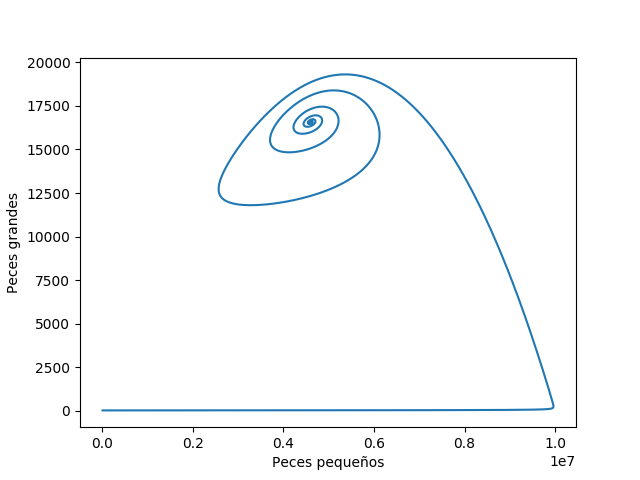
\includegraphics[scale=0.5]{img/ambos-4000-25.png}
\caption{Evolución de la población de peces pequeños y grandes}
\end{figure}

Se puede ver claramente la forma en espiral que tiene. Esto es por lo siguiente: si nos fijamos en las dos gráficas anteriores, vemos cómo
tras crecer la población de pequeños, empieza a disminuir a medida que aumenta la de peces grandes. Cuando no hay suficientes pequeños
para alimentar a los grandes, estos últimos van disminuyendo otra vez, en incremento de los pequeños.

Si superponemos las dos gráficas que representan las poblaciones, se podrá ver todavía mejor (simplemente visual, ya que las cantidades de
peces que tenemos para cada especie son totalmente diferentes).

\begin{figure}[H]
\centering
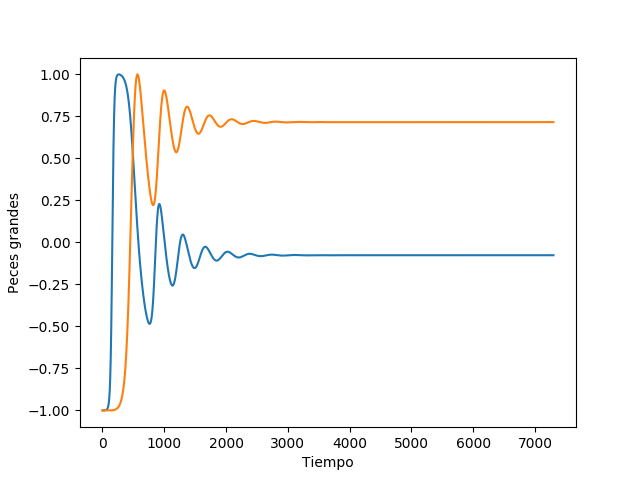
\includegraphics[scale=0.5]{img/interp.png}
\caption{Comparación de las poblaciones}
\end{figure}


\section{Campaña de pesca}

Supongamos ahora que la especie de pez depredador tiene interés comercial, y que se realizarán campañas de pesca en un determinado instante
de tiempo y en las cuales el 50\% de los peces grandes será pescado. Vamos a comprobar cómo afectaría al equilibrio del sistema esta campaña.
Para que se vea bien cómo afecta la pesca al sistema ya equilibrado, la he puesto cada 10 años para que se ejecute justo en mitad de la
simulación, ya que lo teniamos puesto que durase 20 años.

Tras ejecutarlo, este ha sido el resultado:

\begin{figure}[H]
	\begin{minipage}{0.5\textwidth}
	  \centering
	  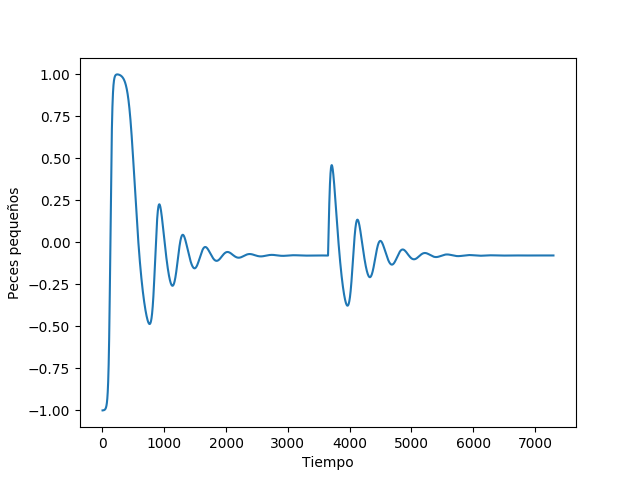
\includegraphics[scale=0.45]{img/pequenios-4000-25-pesca.png}
	\end{minipage}
	\begin{minipage}{0.5\textwidth}
	  \centering
	  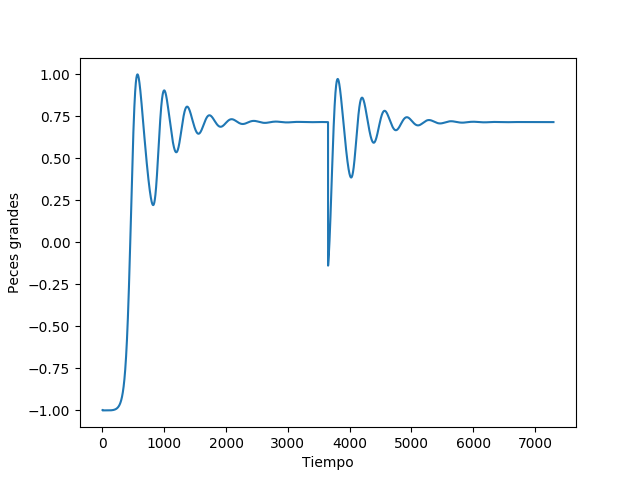
\includegraphics[scale=0.45]{img/grandes-4000-25-pesca.png}
	\end{minipage}
	\caption{Evolución de la población de peces en 7300 días con pequeños: 1000, grandes: 25 y campaña de pesca: 50\%}
\end{figure}

El resultado que obtenemos tras la campaña de pesca es prácticamente el mismo que se obtiene al principio de la ejecución, cuando no están
equilibrados. El número de peces grandes disminuye a la mitad y, en consecuencia, el número de peces pequeños aumenta, ya que no hay tantos
depredadores. Una vez vuelva a crecer el número de peces grandes, el número de peces pequeños disminuirá y así sucesivamente hasta volver
al equilibrio que teníamos.

Si analizamos la gráfica resultante de comparar el número de peces pequeños con el grande, obtenemos lo siguiente:

\begin{figure}[H]
\centering
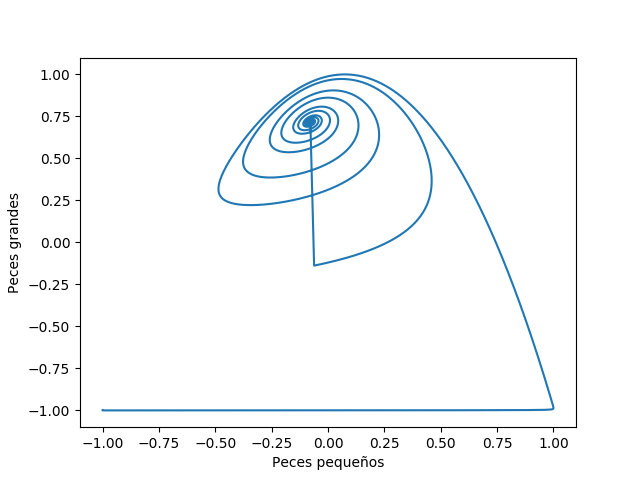
\includegraphics[scale=0.5]{img/ambos-4000-25-pesca.png}
\caption{Evolución de la población de peces pequeños y grandes con campaña de pesca}
\end{figure}

Podemos ver que la gráfica no ha cambiado en exceso. Tenemos un escalón bastante grande por mitad de la espiral, el cual representa la
campaña de pesca realizada. Sin embargo, sigue manteniendo una forma de espiral muy parecida a la que hemos visto anteriormente, es decir,
pese a alterar el sistema, las poblaciones han vuelto a equilibrarse de la misma forma que lo estaban haciendo.

Veamos lo que sucedería si aumentamos la cantidad de peces pescados en la campaña. Pongamos que se pesca un 75\% de los peces grandes. Este
sería el resultado:

\begin{figure}[H]
	\begin{minipage}{0.5\textwidth}
	  \centering
	  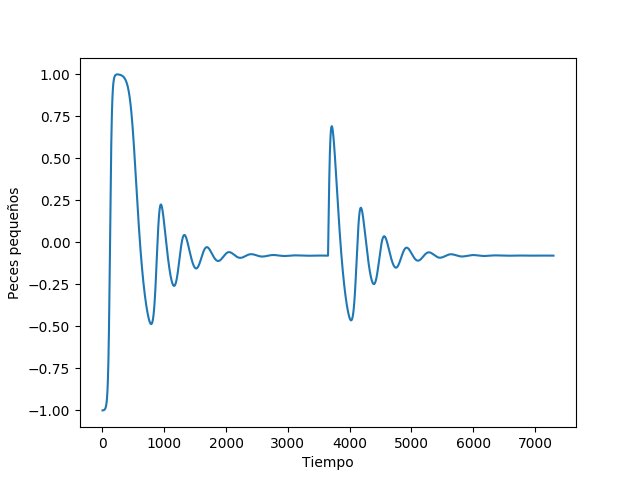
\includegraphics[scale=0.45]{img/pequenios-4000-25-pesca75.png}
	\end{minipage}
	\begin{minipage}{0.5\textwidth}
	  \centering
	  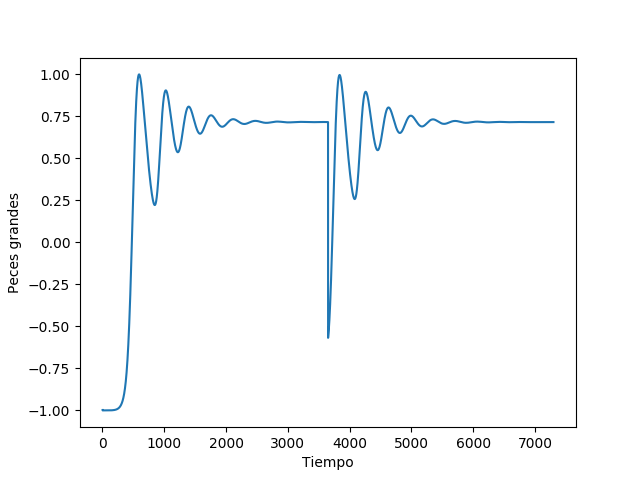
\includegraphics[scale=0.45]{img/grandes-4000-25-pesca75.png}
	\end{minipage}
	\caption{Evolución de la población de peces en 7300 días con pequeños: 1000, grandes: 25 y campaña de pesca: 75\%}
\end{figure}

Se puede comprobar a simple vista que, en esta última gráfica, hay una desviación un poco más alta en cuanto a la cantidad de peces, debida a
que hemos eliminado aun más peces grandes y que, en consecuencia, el número de peces pequeños ha aumentado todavía más.


\section{Investigando diferentes políticas de pesca}

Si partimos de los resultados obtenidos anteriormente, los mejores momentos para una campaña de pesca sería cuando más peces grandes tenemos,
los cuales vienen relativamente después de una campaña. El momento sería cuando todavía están equilibrándose, pero no se han perdido peces
grandes por falta de alimento (peces pequeños). El mayor problema es que si nos equivocamos y hacemos la campaña un poco antes o un poco más
tarde, puede ser que se pesque muy poco o que acabemos con casi tods los peces.

Para que esto no ocurra, vamos a hacer una simulación para varios momentos después de una campaña. También tendremos en cuenta que no partiremos
de la primera vez que metemos los peces en el lago, ya que lo más lógico sería comenzar las campañas una vez ya esté equilibrado todo por primera
vez (que es cuando más tardaría, dependiendo del número de peces echados al principio). Prefiero hacerlo así porque el problema no nos dice si
podemos controlar o no el número de peces inicial, si no también podríamos barajar esa opción

Veamos los resultados que obtenemos con una variación de campañas entre los 2 y los 6 meses pescando el 70\%, 80\% y 90\%:

\begin{figure}[H]
	\begin{minipage}{0.5\textwidth}
	  \centering
	  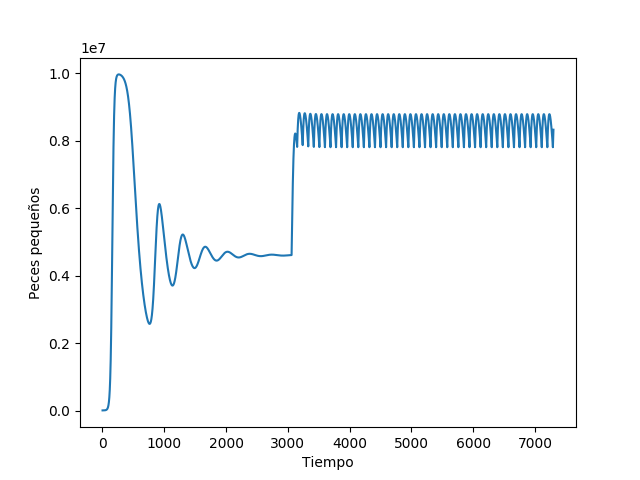
\includegraphics[scale=0.45]{img/pequenios-4000-25-pescapol.png}
	\end{minipage}
	\begin{minipage}{0.5\textwidth}
	  \centering
	  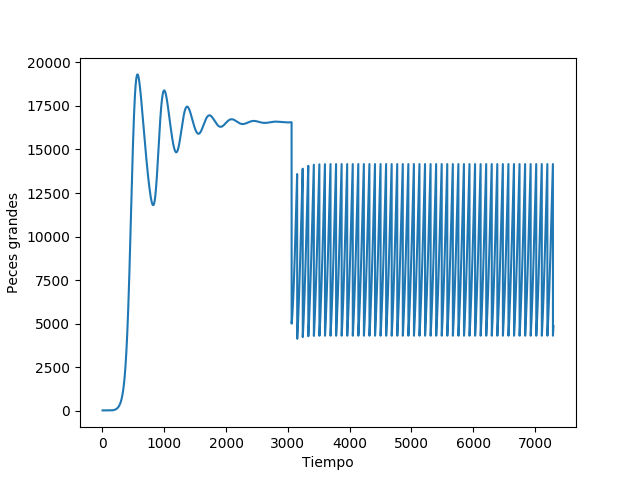
\includegraphics[scale=0.45]{img/grandes-4000-25-pescapol.png}
	\end{minipage}
	\caption{Resultados de la mejor política de pesca}
\end{figure}

\begin{table}[H]
\centering
\resizebox{\textwidth}{!}{%
\begin{tabular}{c|c|c}
\textbf{Meses entre campaña} & \textbf{Porcentaje de peces} & \textbf{Número de peces} \\ \hline
\textbf{2}     	 			 & 70                     		& 217677                   \\
\textbf{2}     	 			 & 80                     		& 263093                   \\
\textbf{2}     	 			 & 90                     		& 20854                    \\ \hline
\textbf{3}     	 		 	 & \textbf{70}                  & \textbf{476841}   	   \\
\textbf{3}     	 		 	 & 80                    		& 340578   	               \\
\textbf{3}     	 		 	 & 90                    		& 33701   	               \\ \hline
\textbf{4}     	 		 	 & 70                    		& 436078   	               \\
\textbf{4}     	 		 	 & 80                    		& 438955   	               \\
\textbf{4}     	 		 	 & 90                    		& 253930   	               \\ \hline
\textbf{5}     	 		 	 & 70                   		& 372296   	               \\ 
\textbf{5}     	 		 	 & 80                    		& 411514   	               \\ 
\textbf{5}     	 		 	 & 90                    		& 381355   	               \\ \hline
\textbf{6}	     			 & 70                      		& 320225                   \\ 
\textbf{6}	     			 & 80                      		& 367629                   \\ 
\textbf{6}	     			 & 90                      		& 392488                   \\ 
\end{tabular}%
}
\end{table}

Podemos ver que la mejor política ha sido una pesca cada 3 meses del 70\% de los peces, la cual podemos ver en la gráfica cómo va cambiando
la población regularmente. En ella podemos comprobar como lo que hemos dicho antes puede no ser del todo cierto, y es que realizar la pesca
cuando hay más peces, no garantiza que se pesque más.

Esto se debe a que, por mucho peces que haya, si realizo una pesca muy grande, tendré que esperar más tiempo a que vuelva a haber una
cantidad considerable de estos. No obstante, si pesco una cantidad más reducida, tardaré menos en poder volver a pescar una cantidad semejante.

También podemos ver en la tabla como los valores tienen muy poco que ver entre unos porcentajes y otros. Se puede ver que, tanto pescar mucho
porcentaje y esperar más, como pescar un porcentaje menor y esperar menos, pueden ofrecer unos resultados bastante aceptables. En mi caso,
yo me quedaría con pescar menos, porque el número de peces que se pescan no tienen una varianza tan grande en comparación con los otros, y
además, te arriesgas menos a extinguir la especie. 


\end{document}

